\documentclass[../informe2.tex]{subfiles}
\begin{document}

Que fue lo que se logró con la experimentación, incluir tablas y parámetros,
gráficos, etc.\ lo más explicativo posible. Además destacar puntos
importantes del problema, características de las instancias que influyeron
en los resultados, valores de parámetros que influyeron en los resultados,
análisis de calidad de las soluciones encontradas a través del tiempo,
análisis en profundidad de la técnica vs los resultados obtenidos,
valores promedio, desviaciones, \textbf{comparaciones con resultados
	de la literatura}, etc. También debería discutir qué cosas podría
haber agregado o quedan como desafíos para trabajo futuro en su algoritmo.


\begin{table}[h]
	\small
	\makebox[\textwidth][c]{
		\begin{tabular}{@{}lrrrrrrrrrr@{}}
			\toprule
			Estadística/Instancia                       & a1\_1 & a1\_2 & a1\_3 & a1\_4 & a1\_5 & a2\_1  & a2\_2 & a2\_3 & a2\_4 & a2\_5 \\ \midrule
			Total de servicios                          & 79    & 980   & 216   & 142   & 981   & 1000   & 170   & 129   & 180   & 153   \\
			\begin{tabular}[c]{@{}l@{}}Servicios sin dependencias\\ y spreadmin nulo\end{tabular} & 73    & 970   & 116   & 44    & 972   & 1000   & 92    & 4     & 55    & 29    \\
			\%                                          & 92.41 & 98.98 & 53.70 & 30.99 & 99.08 & 100.00 & 54.12 & 3.10  & 30.56 & 18.95 \\ \bottomrule
		\end{tabular}}
\end{table}

\begin{table}[h]
	\small
	\makebox[\textwidth][c]{
		\begin{tabular}{@{}lrrrrrrrrrr@{}}
			\toprule
			Estadística/Instancia                                                                 & b\_1  & b\_2  & b\_3  & b\_4  & b\_5  & b\_6  & b\_7  & b\_8  & b\_9  & b\_10 \\ \midrule
			Total de servicios                                                                    & 2512  & 2462  & 15025 & 1732  & 35082 & 14680 & 15050 & 45030 & 4609  & 4896  \\
			\begin{tabular}[c]{@{}l@{}}Servicios sin dependencias\\ y spreadmin nulo\end{tabular} & 2012  & 1962  & 14025 & 732   & 34082 & 13680 & 14050 & 44030 & 3609  & 3896  \\
			\%                                                                                    & 80.10 & 79.69 & 93.34 & 42.26 & 97.15 & 93.19 & 93.36 & 97.78 & 78.30 & 79.58 \\ \bottomrule
		\end{tabular}}
		\caption{\small Por cada instancia, se determina la cantidad de servicios que no poseen dependencias y tienen un mínimo de dispersión igual a cero.}\label{tabla:analisis-servicios}
\end{table}

\begin{table}[h]
	\small
	\makebox[\textwidth][c]{
	\begin{tabular}{@{}lrrrrrrrrrr@{}}
		\toprule
		Estadística/Instancia       & a1\_1 & a1\_2 & a1\_3 & a1\_4 & a1\_5 & a2\_1 & a2\_2 & a2\_3 & a2\_4 & a2\_5 \\ \midrule
		Total de procesos           & 100   & 1000  & 1000  & 1000  & 1000  & 1000  & 1000  & 1000  & 1000  & 1000  \\
		Procesos asignados          & 98    & 956   & 116   & 843   & 974   & 1000  & 945   & 4     & 62    & 58    \\
		Tiempo de ejecución [s] & 0     & 0     & 0     & 0     & 0     & 0     & 1     & 0     & 0     & 1     \\ %\bottomrule
	\end{tabular}}

	\bigskip

	\makebox[\textwidth][c]{
	\begin{tabular}{@{}lrrrrrrrrrr@{}}
		%\toprule
		Estadística/Instancia       & b\_1 & b\_2 & b\_3  & b\_4  & b\_5  & b\_6  & b\_7  & b\_8  & b\_9  & b\_10 \\ \midrule
		Total de procesos           & 5000 & 5000 & 20000 & 20000 & 40000 & 40000 & 40000 & 50000 & 50000 & 50000 \\
		Procesos asignados          & 2012 & 1962 & 14025 & 732   & 34082 & 13680 & 14050 & 44030 & 3609  & 3896  \\
		Tiempo de ejecución [s] & 2    & 2    & 8     & 26    & 22    & 26    & 300   & 29    & 117   & 300   \\ \bottomrule
	\end{tabular}}
	\caption{\small Por cada instancia, se muestra el número de procesos asignados con el algoritmo \textit{Greedy}.}\label{tabla:greedy}
\end{table}


\begin{table}[h]
	\footnotesize
	\makebox[\textwidth][c]{
\begin{tabular}{@{}lrrrrrrrr@{}}
\toprule
Instancia & Inicial & HC & Tiempo & Iteraciones & HC-SP & Tiempo & Iteraciones & Diferencia \\ \midrule
a1\_1     & 49528750                    & 44307612               & 0                          & 200                             & 44306501                  & 0                          & 200                             & -1111                          \\
a1\_2     & 1061649570                  & 878229613              & 1                          & 3000                            & 929137945                 & 0                          & 2000                            & 50908332                       \\
a1\_3     & 583662270                   & 583384296              & 1                          & 3000                            & 583373392                 & 1                          & 2000                            & -10904                         \\
a1\_4     & 632499600                   & 570401602              & 0                          & 2000                            & 568344744                 & 0                          & 2000                            & -2056858                       \\
a1\_5     & 782189690                   & 728145497              & 1                          & 4000                            & 737253098                 & 1                          & 3000                            & 9107601                        \\
a2\_1     & 391189190                   & 35481989               & 4                          & 7000                            & 38489889                  & 4                          & 5000                            & 3007900                        \\
a2\_2     & 1876768120                  & 1494274528             & 2                          & 7000                            & 1415300243                & 0                          & 3000                            & -78974285                      \\
a2\_3     & 2272487840                  & 1869593233             & 1                          & 5000                            & 1734732392                & 1                          & 3000                            & -134860841                     \\
a2\_4     & 3223516130                  & 2283923795             & 3                          & 9000                            & 2128654638                & 3                          & 8000                            & -155269157                     \\
a2\_5     & 787355300                   & 650311032              & 2                          & 9000                            & 612089208                 & 2                          & 8000                            & -38221824                      \\
b\_1      & 7644173180                  & 5271411947             & 10                         & 20000                           & 5314076290                & 7                          & 15000                           & 42664343                       \\
b\_2      & 5181493830                  & 1278123023             & 91                         & 60000                           & 1150616078                & 110                        & 70000                           & -127506945                     \\
b\_3      & 6336834660                  & 1149013744             & 248                        & 180000                          & 1953270617                & 64                         & 80000                           & 804256873                      \\
b\_4      & 9209576380                  & 4679312094             & 300                        & 30489                           & 4678242633                & 300                        & 30887                           & -1069461                       \\
b\_5      & 12426813010                 & 2968606165             & 300                        & 48269                           & 3252021891                & 298                        & 200000                          & 283415726                      \\
b\_6      & 12749861240                 & 9526211153             & 300                        & 42377                           & 9526194551                & 300                        & 43333                           & -16602                         \\
b\_7      & 37946901700                 & 31761671090            & 300                        & 4872                            & 18067048987               & 300                        & 10248                           & -13694622103                   \\
b\_8      & 14068207250                 & 6651200779             & 300                        & 21484                           & 5314963613                & 300                        & 95278                           & -1336237166                    \\
b\_9      & 23234641520                 & 16030720890            & 300                        & 9337                            & 15896062116               & 300                        & 17959                           & -134658774                     \\
b\_10     & 42220868760                 & 38023415516            & 300                        & 3620                            & 20990879440               & 300                        & 9822                            & -17032536076                   \\ \bottomrule
\end{tabular}}
\caption{\small Detalle de los resultados obtenidos, utilizando las dos versiones del algoritmo \textit{Hill Climbing}.}\label{tabla:hc-comparative}
\end{table}


\begin{figure}[ht]
	\makebox[\textwidth][c]{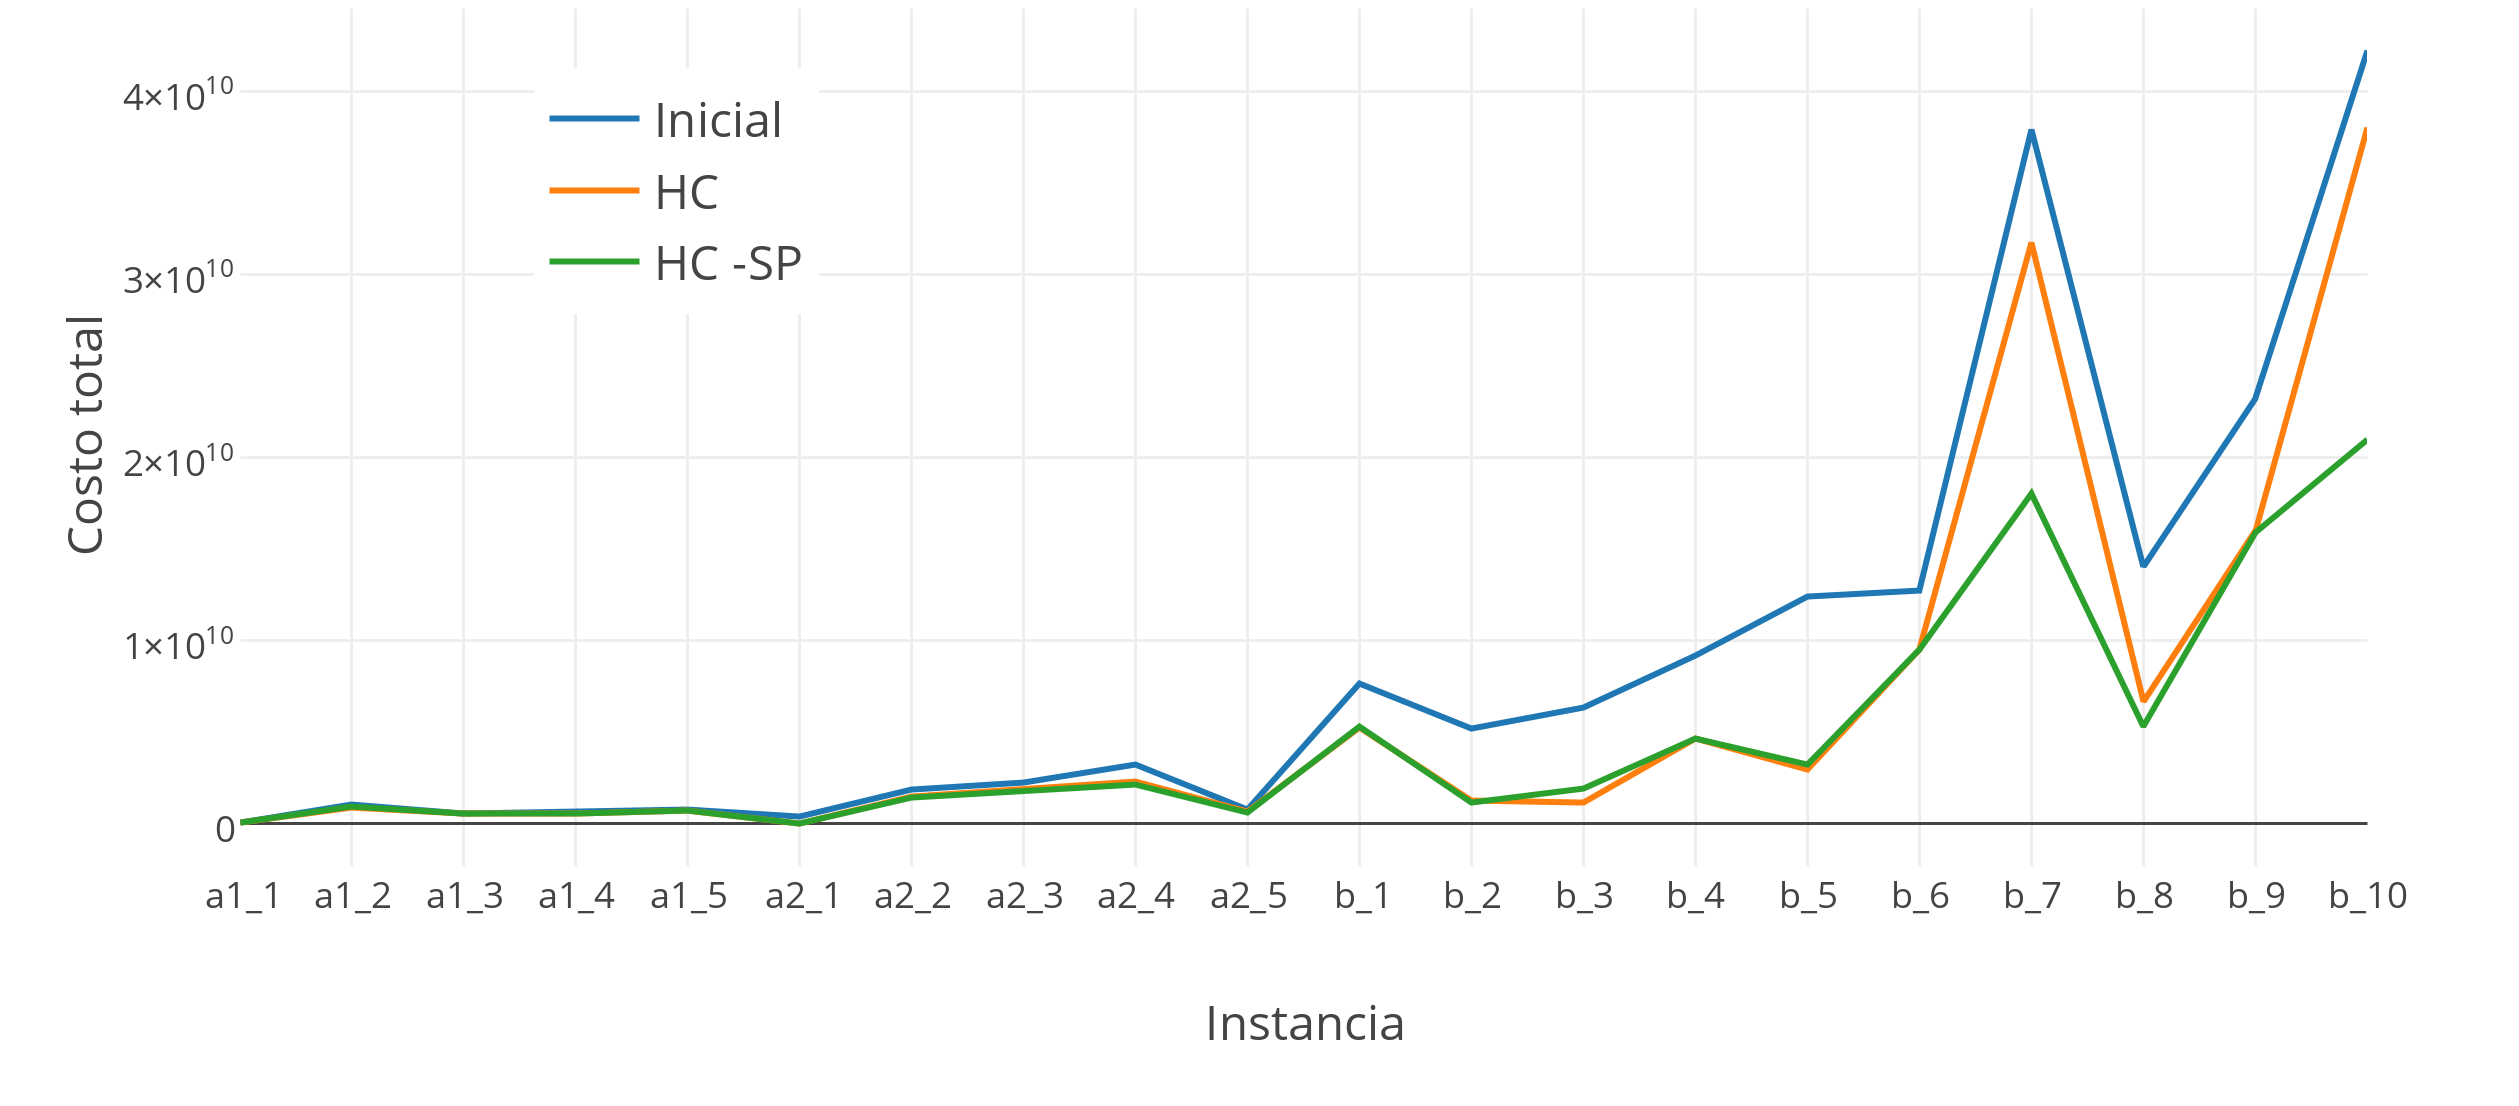
\includegraphics[width=1.2\textwidth]{comparativa-hc.png}}
	\caption{\small}\label{fig:comparativa-hc}
\end{figure}


\begin{table}[h]
	\small
\centering
\begin{tabular}{@{}lrrr@{}}
\toprule
Modelo & Inicial & Mejor ROADEF 2012 & HC-SP \\ \midrule
a1\_1  & 49528750               & 44306501            & 44306501              \\
a1\_2  & 1061649570             & 777532896           & 929137945             \\
a1\_3  & 583662270              & 583005717           & 583373392             \\
a1\_4  & 632499600              & 252728589           & 568344744             \\
a1\_5  & 782189690              & 727578309           & 737253098             \\
a2\_1  & 391189190              & 198                 & 38489889              \\
a2\_2  & 1876768120             & 816523983           & 1415300243            \\
a2\_3  & 2272487840             & 1306868761          & 1734732392            \\
a2\_4  & 3223516130             & 1681353943          & 2128654638            \\
a2\_5  & 787355300              & 336170182           & 612089208             \\
b\_1   & 7644173180             & 3339186879          & 5314076290            \\
b\_2   & 5181493830             & 1015553800          & 1150616078            \\
b\_3   & 6336834660             & 156835787           & 1953270617            \\
b\_4   & 9209576380             & 4677823040          & 4678242633            \\
b\_5   & 12426813010            & 923092380           & 3252021891            \\
b\_6   & 12749861240            & 9525857752          & 9526194551            \\
b\_7   & 37946901700            & 14835149752         & 18067048987           \\
b\_8   & 14068207250            & 1214458817          & 5314963613            \\
b\_9   & 23234641520            & 15885486698         & 15896062116           \\
b\_10  & 42220868760            & 18048515118         & 20990879440           \\ \bottomrule
\end{tabular}
\caption{\small Por cada instancia se presentan, el mejor resultado obtenido en el desafío de la ROADEF 2012 y el conseguido con \textit{HC-SP}.}
\label{tabla:comparative-with-best-roadef}
\end{table}



\begin{figure}[ht]
	\makebox[\textwidth][c]{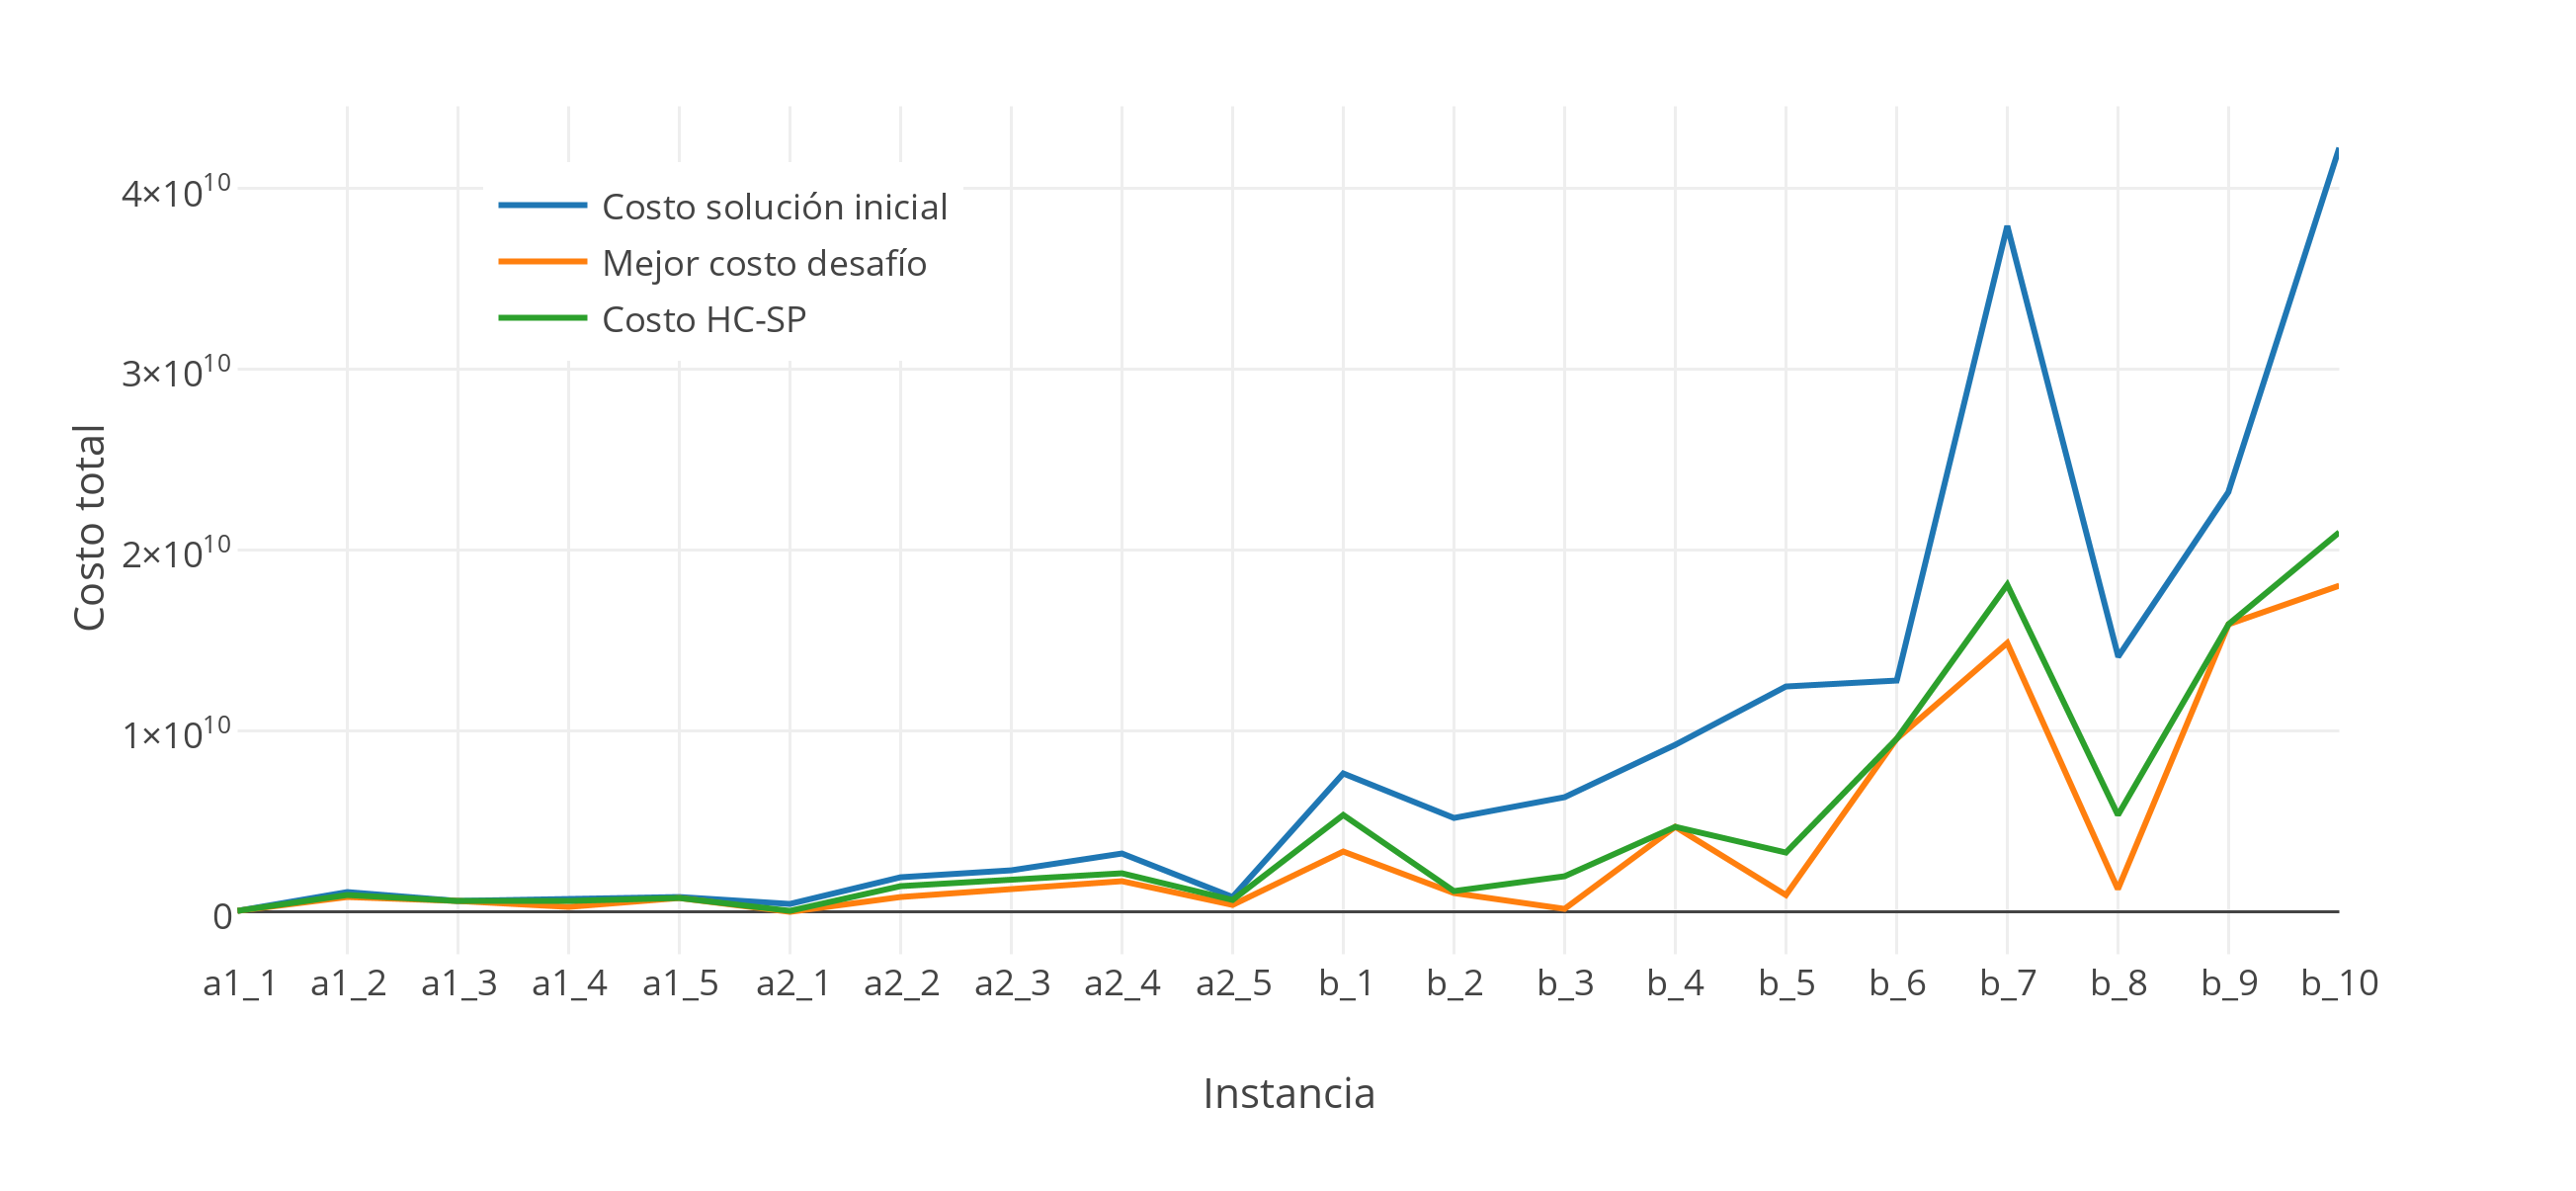
\includegraphics[width=1.2\textwidth]{comparativa-hc-best-challenge.png}}
	\caption{\small}\label{fig:comparativa-hc-best-challenge}
\end{figure}


\end{document}
